\documentclass[10pt,a4paper,oneside]{book}
\usepackage[left=1.5cm,top=1.5cm,right=1.5cm,bottom=1.5cm]{geometry}
			
\usepackage[english]{babel}
\usepackage[utf8]{inputenc}
\usepackage[protrusion=true,expansion=true]{microtype}
\usepackage{amsmath,amsfonts,amsthm}     % Math packages
\usepackage{graphicx}                    % Enable pdflatex
\usepackage[svgnames]{xcolor}            % Colors by their 'svgnames'
\usepackage{geometry}
\usepackage[colorlinks=true,linkcolor=blue,urlcolor=blue]{hyperref}
\usepackage{wrapfig}
\usepackage{fontawesome}
\usepackage{attachfile}

\let\olditemize\itemize
\def\itemize{\olditemize\itemsep=0pt }

\showoutput
\showboxdepth=3
\frenchspacing              % Better looking spacings after periods
\pagestyle{empty}           % No pagenumbers/headers/footers


%%% Custom sectioning}{sectsty package)
%%% ------------------------------------------------------------
\usepackage{sectsty}

\sectionfont{%			            % Change font of \section command
	\usefont{OT1}{phv}{b}{n}%		% bch-b-n: CharterBT-Bold font
	\sectionrule{0pt}{0pt}{-5pt}{3pt}}

%%% Macros
%%% ------------------------------------------------------------
\newlength{\spacebox}
\settowidth{\spacebox}{8888888888}			% Box to align text
\newcommand{\sepspace}{\vspace*{0pt}}		% Vertical space macro

\newcommand{\MyName}[1]{ % Name
		\Huge \usefont{OT1}{phv}{b}{n} \hfill #1
		\par \normalsize \normalfont}
		
\newcommand{\MySlogan}[1]{ % Slogan}{optional)
		\large 
		\hfill #1
		\par \normalsize \normalfont}

\newcommand{\NewPart}[2]{\section*{\uppercase{#1} #2}}

\newcommand{\PersonalEntry}[2]{
		\noindent\hangindent=2em\hangafter=0 % Indentation
		\parbox{\spacebox}{        % Box to align text
		\textit{#1}}		       % Entry name}{birth, address, etc.)
		\hspace{1.5em} #2 \par}    % Entry value

\newcommand{\SkillsEntry}[2]{      % Same as \PersonalEntry
		\noindent\hangindent=2em\hangafter=0 % Indentation
		\parbox{\spacebox}{        % Box to align text
		\textit{#1}}			   % Entry name}{birth, address, etc.)
		\hspace{1.5em} #2 \par}    % Entry value	
		
\newcommand{\EducationEntry}[4]{	
		\noindent \textbf{#1} \hfill    % Study
			\parbox[t][][b]{0.2\textwidth}{%
			\hfill\color{Black}#2} \par  % Duration
		\noindent \textit{#3} \par        % School
		\noindent\hangindent=1.5em\hangafter=0 \small #4 % Description
		\normalsize \par}

\newcommand{\EducationEntrya}[4]{\noindent\ignorespaces	
		\begin{minipage}[t][][b]{0.8\textwidth} \raggedright{\textbf{#1}} \end{minipage} \hfill 
		\begin{minipage}[t][][b]{0.2\textwidth} \hfill\color{Black}#2 \end{minipage} 
		 
		\noindent \textit{#3} \par        % School
		\noindent\hangindent=2em\hangafter=0 \small #4 
		\normalsize \par}
		
\newcommand{\LanguageEntry}[2]{\noindent\ignorespaces
\textbf{#1}	\par
\noindent \small #2 \par
}

\newcommand{\WorkEntry}[4]{				  % Same as \EducationEntry
		\noindent \textbf{#1} \hfill      % Jobname
		\colorbox{White}{\color{White}#2} \par  % Duration
		\noindent \textit{#3} \par              % Company
		\noindent\hangindent=2em\hangafter=0 \small #4 % Description
		\normalsize \par}
		
\newcommand{\VolunteeringEntry}[3]{	\noindent\ignorespaces						
		\begin{minipage}[t][][b]{0.8\textwidth} \raggedright{\textbf{#1}} \end{minipage} \hfill 
		\begin{minipage}[t][][b]{0.2\textwidth} \hfill\color{Black}#2 \end{minipage} 
		 
		\noindent \textit{#3} \par        % School
		}
\newcommand{\ITSkillEntry}[2]{\noindent\ignorespaces
\textbf{#1}	\par
\noindent \small #2 \par
}

\newcommand{\PaperEntry}[7]{
		\noindent #1, ``\href{#7}{#2}", \textit{#3} \textbf{#4}, #5 (#6).}

\newcommand{\ArxivEntry}[3]{
		\noindent #1, ``\href{http://arxiv.org/abs/#3}{#2}", \textit{{cond-mat/}#3}.}
        
\newcommand{\BookEntry}[4]{
		\noindent #1, ``\href{#3}{#4}", \textit{#3}.}
        
\newcommand{\FundingEntry}[5]{
        \noindent #1, ``#2", \$#3 (#4, #5).}

\newcommand{\TalkEntry}[4]{
		\noindent #1, #2, #3 #4}

\newcommand{\ThesisEntry}[5]{
		\noindent #1 -- #2 #3 ``#4" \textit{#5}}

\newcommand{\CourseEntry}[3]{
		\noindent \item{#1: \textbf{#2} \\ #3}}
%%% Begin Document
%%% ------------------------------------------------------------
\begin{document}

%\layout

% you can upload a photo and include it here...
\begin{wrapfigure}{l}{0.2\textwidth}
	\vspace*{-2em}
		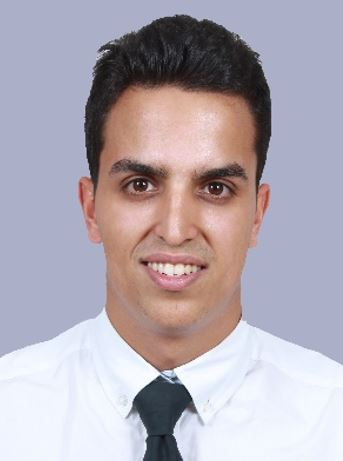
\includegraphics[width=.19\textwidth]{Assets/picture.JPG}
\end{wrapfigure}

\MyName{Álvaro Zornoza Uña}
\MySlogan{\vspace{-0.15in}\begin{flushright} 
\hfill Industrial Electronics, Robotics and Automation Engineering \\ Madrid (Spain) \\ +34 693 803 083 \\ 
\href{mailto:alvaro.zornoza@gmail.com}{alvaro.zornoza@gmail.com} \\ \href{https://www.linkedin.com/in/alvaro-zornoza/}{ \faLinkedin} Alvaro Zornoza Uña \\ \href{https://github.com/alvarozornoza}{ \faGithub} alvarozornoza \\ 
\end{flushright}}

\vspace{0.01in}
\sepspace
 \NewPart{Overview}{}
 
 \begin{itemize}
 \item My main areas of interest are robotics, drones, embedded systems, IoT, AI and computer vision.
 \item I consider myself a responsible, hard-working and organised person. I am always eager to learn new things. Extracurricular activities carried out during my bachelor's degree have provided me with good communication, teamwork and leadership skills.
 \end{itemize}

%%% Work experience
%%% ------------------------------------------------------------
\NewPart{Work Experience}{}

\EducationEntrya{R\&D Engineer Intern}{Mar 2019 - Sep 2019}{Siemens AG (Graz)}{\begin{itemize} 
\item Internship at the Development House of the Digital Factory department. 
\item Writing the master thesis in the framework of Predictive Maintenance.
\item Firmware development for STM32 microcontrollers and automation projects for Simatic STEP 7-1500 with TIA Portal\end{itemize}}
\sepspace

\EducationEntrya{Computer Vision Graduate Researcher}{Oct 2018 - Feb 2019}{Polytechnic University of Catalonia - BarcelonaTech (Barcelona)}{\begin{itemize} 
\item Participating in the European project Personal Online Dosimetry Using Computational Methods. \href{https://podium-concerth2020.eu}{PODIUM} project is part of \href{http://www.concert-h2020.eu/}{CONCERT} European Joint Programme for the Integration of Radiation Protection Research under Horizon 2020.
\item Integrating multiple RGB-D cameras for 3-D human body localization and tracking (Visual Studio, C++, C\#, OpenCV)
\end{itemize}}
\sepspace

\EducationEntrya{IoT Application Engineer and Consultant}{Apr 2018 - Oct 2018}{\href{https://thethings.io/}{thethings.iO} (Barcelona)}{\begin{itemize} 
\item Integrating third-party services (APIs REST) with the platform (HTTP, CoAP \& UDP and MQTT protocols).
\item Prior knowledge of Web applications development (Angular, NodeJS and MongoDB)
\item Supporting customers with the setup of IoT projects and programming of cloud-code scripts (NodeJS).
\item Representing on behalf of the company for projects and meetings with other customers and institutions.
\end{itemize}}
\sepspace

\EducationEntrya{Intern}{Sep 2017 - Apr 2018}{\href{https://thethings.io/}{thethings.iO} (Barcelona)}{\begin{itemize}
\item Programming libraries for embedded-system (C++, Arduino, Python)
\item Integrating services of Sigfox and other LPWAN technologies with the platform.
\item Writing website content for both the blog and  documentation of the platform. 
\end{itemize}}
\sepspace

\EducationEntrya{Assistant Laboratory Technician}{Feb 2017 - Jul 2017}{Kaunas University of Technology (Lithuania)}{\begin{itemize} 
\item Internship at \href{https://fablabkaunas.lt/}{FabLAB Kaunas} while an Erasmus + Exchange assisting for scientific research. 
\item Commissioning and maintenance of simulation equipment.  Documentation and programming of DJI drones.
\end{itemize}}
\sepspace

%%% Education
%%% ------------------------------------------------------------
\NewPart{Education and training}{}

\EducationEntrya{Master’s Degree in Automatic Control and Robotics }{Sep 2017 - Sep 2019}{Polytechnic University of Catalonia - BarcelonaTech (Spain)}{\begin{itemize}
\item 120 ECTS credits. %GPA: 
\item Honours in Human Robot Interaction and Teleoperation.
\item Erasmus+ Exchange at Graz University of Technology (Austria) during last semester.
\item Master's thesis: \href{https://drive.google.com/drive/folders/16OLXcMPocBu6cA3fjj0tfiSJJ1OARVSW?usp=sharing}{Enabling fault prediction of electromechanical relays by incorporating accelerated life tests using Siemens SIMATIC safety controllers}.
\end{itemize}}

\sepspace
\EducationEntrya{Bachelor's Degree in Industrial Electronics and Automation Engineering
\\}{Sep 2013 - Jul 2017}{Technical University of Madrid (Spain)}{\begin{itemize} \item 240 ECTS credits. GPA: 7.1/10 (B). \item Honours in Physics I and Business Management. 
\item Erasmus+ Exchange at Kaunas University of Technology (Lithuania) during last semester.
\item Outstanding (A+) grade in Bachelor's Thesis: \href{https://drive.google.com/drive/folders/0BxCxXmj96TUnUUFpQUlhY3JpNTQ?usp=sharing}{Design of a Drone Based  Measurement System for GSM signals}.\end{itemize}}
\sepspace

% \EducationEntrya{Bachelor's Degree in Electronics Engineering}{Feb 2017 - Jul 2017}{Erasmus+ Exchange at Kaunas University of Technology (Lithuania)}{\begin{itemize}\item Internship at the laboratory in \href{https://fablabkaunas.lt/}{FabLAB Kaunas}. \item Writing the Bachelor's thesis and attending several elective courses. \end{itemize}}
\sepspace

%%% Conferences, courses and seminars
%%% ------------------------------------------------------------
\NewPart{Conferences, courses and seminars}{}
\EducationEntrya{Digital Signal and Image Processing with MATLAB}{Nov 2016}{Czech Technical University in Prague (Czech Republic)}{}
\EducationEntrya{Organisational Behaviour}{Sep 2015}{Technical University of Madrid (Spain)}{\begin{itemize}\item Seminar on Organisational Behaviour for mentorship training.
\item Learning communication and motivation skills and how to make efficient presentations. \end{itemize}}

%%% Languages
%%% ------------------------------------------------------------
\NewPart{Languages}{}
\LanguageEntry{Spanish}{Native speaker}
\sepspace
\LanguageEntry{English}{Professional working proficiency. C1 - British Council Aptis English Test}
\sepspace
\LanguageEntry{German}{Elementary proficiency. A1 - University of Graz (Austria)}

%%% IT skills
%%% ------------------------------------------------------------
\NewPart{Skills}{}
\ITSkillEntry{Programming languages}{C,  C++, C\#, Python, MATLAB \& Simulink, VHDL (FPGA), NodeJS, GScript, API REST and \TeX}
\ITSkillEntry{Robotics framework}{ROS}
\sepspace
\ITSkillEntry{PLC programming}{Siemens S7-1500 and S7-1200. TIA Portal}
\sepspace
\ITSkillEntry{Electronic circuit simulator and PCB design}{Eagle, PSpice and OrCAD}
\sepspace
\ITSkillEntry{CAD programs}{AutoCAD and Inventor}
\sepspace
\ITSkillEntry{Office automation}{MS Office and G Suite}


%%% Honors-Awards
%%% ------------------------------------------------------------
\NewPart{Honors-Awards}{}
\begin{itemize}
    \item Winner of the hackathon \href{https://www.seatdisrup.com/}{SEAT DisrUp: Hacking the Future of Mobility} \hfill April 2018
\end{itemize}


%%% Other Relevant Experience/Skills
%%% ------------------------------------------------------------
\NewPart{Other Relevant Experience/Skills}{}
\begin{itemize}
\item Coordinator at ESN UPC (Barcelona). Organizing events and activities for new incoming students.
\item Basketball Referee for Basketball Association of Madrid. Officiating basketball games during five seasons. Capabilities such as empathy, conflict resolution and teamwork under pressure.
\item Secretary of an University Association: Mountain an Leisure Activities Club of UPM (Madrid). Institutional relations, corporate image and groups management.
\item Mentoring program for new students at University. Providing experience, socialization and personal support to facilitate a good starting experience and beyond.
\item Volunteer experience in several sports events, such as Euroleague Final Four at Madrid (2015) and King’s Cup of Basketball at Malaga (2014).
\item Driver's license (B) and own car.
\end{itemize}

\end{document}